\subsection*{Diametro di un grafo non orientato (\texttt{diametro})}

Vi viene dato in input un grafo non orientato. Dovete trovare la coppia di nodi più lontani e stamparne la distanza.

\paragraph{Formato dell'input}
La prima riga del file di input contiene due interi, \(N\) e \(M\).
\(N\) è il numero di nodi, \(M\) il numero di archi.
Le successive \(M\) righe contengono due interi per riga, i due nodi collegati dall’arco.

\paragraph{Formato dell'output}
L'output deve contenere un intero, uguale alla massima distanza fra due nodi.

% \inputminted[firstline=7]{{assets/codes/diametro.cpp}
% caption = {\texttt{diametro}}

\paragraph{Riferimenti utili}

\begin{itemize}
	\item \texttt{front()} \href{http://www.cplusplus.com/reference/queue/queue/front}{\ExternalLink}
\end{itemize}

\begin{figure}
\centering
\begin{subfigure}[b]{.45\linewidth}
	\begin{figure}[H]\centering
		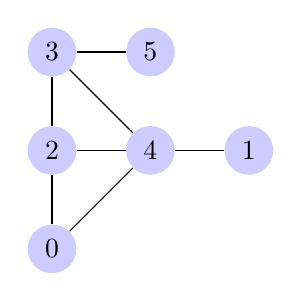
\begin{tikzpicture}[
				scale=.25,
				auto=left,
				every node/.style={circle,fill=blue!20}
			]
			\node (n0) at (5, 0)	{0};
			\node (n1) at (15,5)	{1};
			\node (n2) at (5, 5)	{2};
			\node (n3) at (5, 10)	{3};
			\node (n4) at (10,5)	{4};
			\node (n5) at (10,10)	{5};

			\foreach \from/\to in {
				n0/n2,
				n0/n4,
				n1/n4,
				n2/n4,
				n3/n2,
				n3/n4,
				n3/n5}
				\draw (\from) -- (\to);

		\end{tikzpicture}
	\end{figure}
	\caption{Rappresentazione grafica}
	\label{fig:grafo}
\end{subfigure}
\begin{subfigure}[b]{.45\linewidth}
	\begin{figure}[H]
		\centering
		\begin{tikzpicture}
			\matrix (M) [%
				matrix of nodes,
				column sep = 0pt,
				row sep = 0pt,
				nodes = {draw,
						fill = blue!20,
						minimum width = .5cm,
						outer sep = 0pt,
						minimum height = .5cm,
						anchor = center},
				column 1/.style = {minimum height = .8cm}
			]{
				\mbox{} &[2mm] 2 & \mbox{4} \\
				\mbox{} & 4 & \\
				\mbox{} & 0 & \mbox{3} & \mbox{4} \\
				\mbox{} & 2 & \mbox{4} & \mbox{5} \\
				\mbox{} & 0 & \mbox{1} & \mbox{2} & \mbox{3} \\
				\mbox{} & 3 \\
			};

			\foreach \i in {1, ..., 6} {
				\path (M-\i-1) [late options = {label = center:\i}];
				\draw[->] (M-\i-1.east) -- (M-\i-2.west);
			}
		\end{tikzpicture}
	\end{figure}
	\caption{Rappresentazione tramite lista di adicenza}
	\label{fig:grafo}
\end{subfigure}
\caption{Grafo orientato}
\end{figure}
